\section{}

\subsection{a) Suitable solutioning temperature and extent of the heat treatment window, and b) primary ageing temperature for new alloy}

In figure \ref{fig:diagram05} the amount of all phases is plotted as a function of temperature for the alloy system. Figure \ref{fig:5_01} shows that the $\gamma'$ curve starts at a composition near $0.8$ value and decreases as the temperature increases, reaching a composition of value $0$ around $1380$°C. This temperature is the solutioning temperature. 

For the Liquid curve, it appears at an approximate temperature of $1370$°C, this temperature corresponds to the solidus area. 
The heat treatment window is from the solutioning to the solidus temperature, which is aproximately.

\begin{figure}[h]
  \centering
    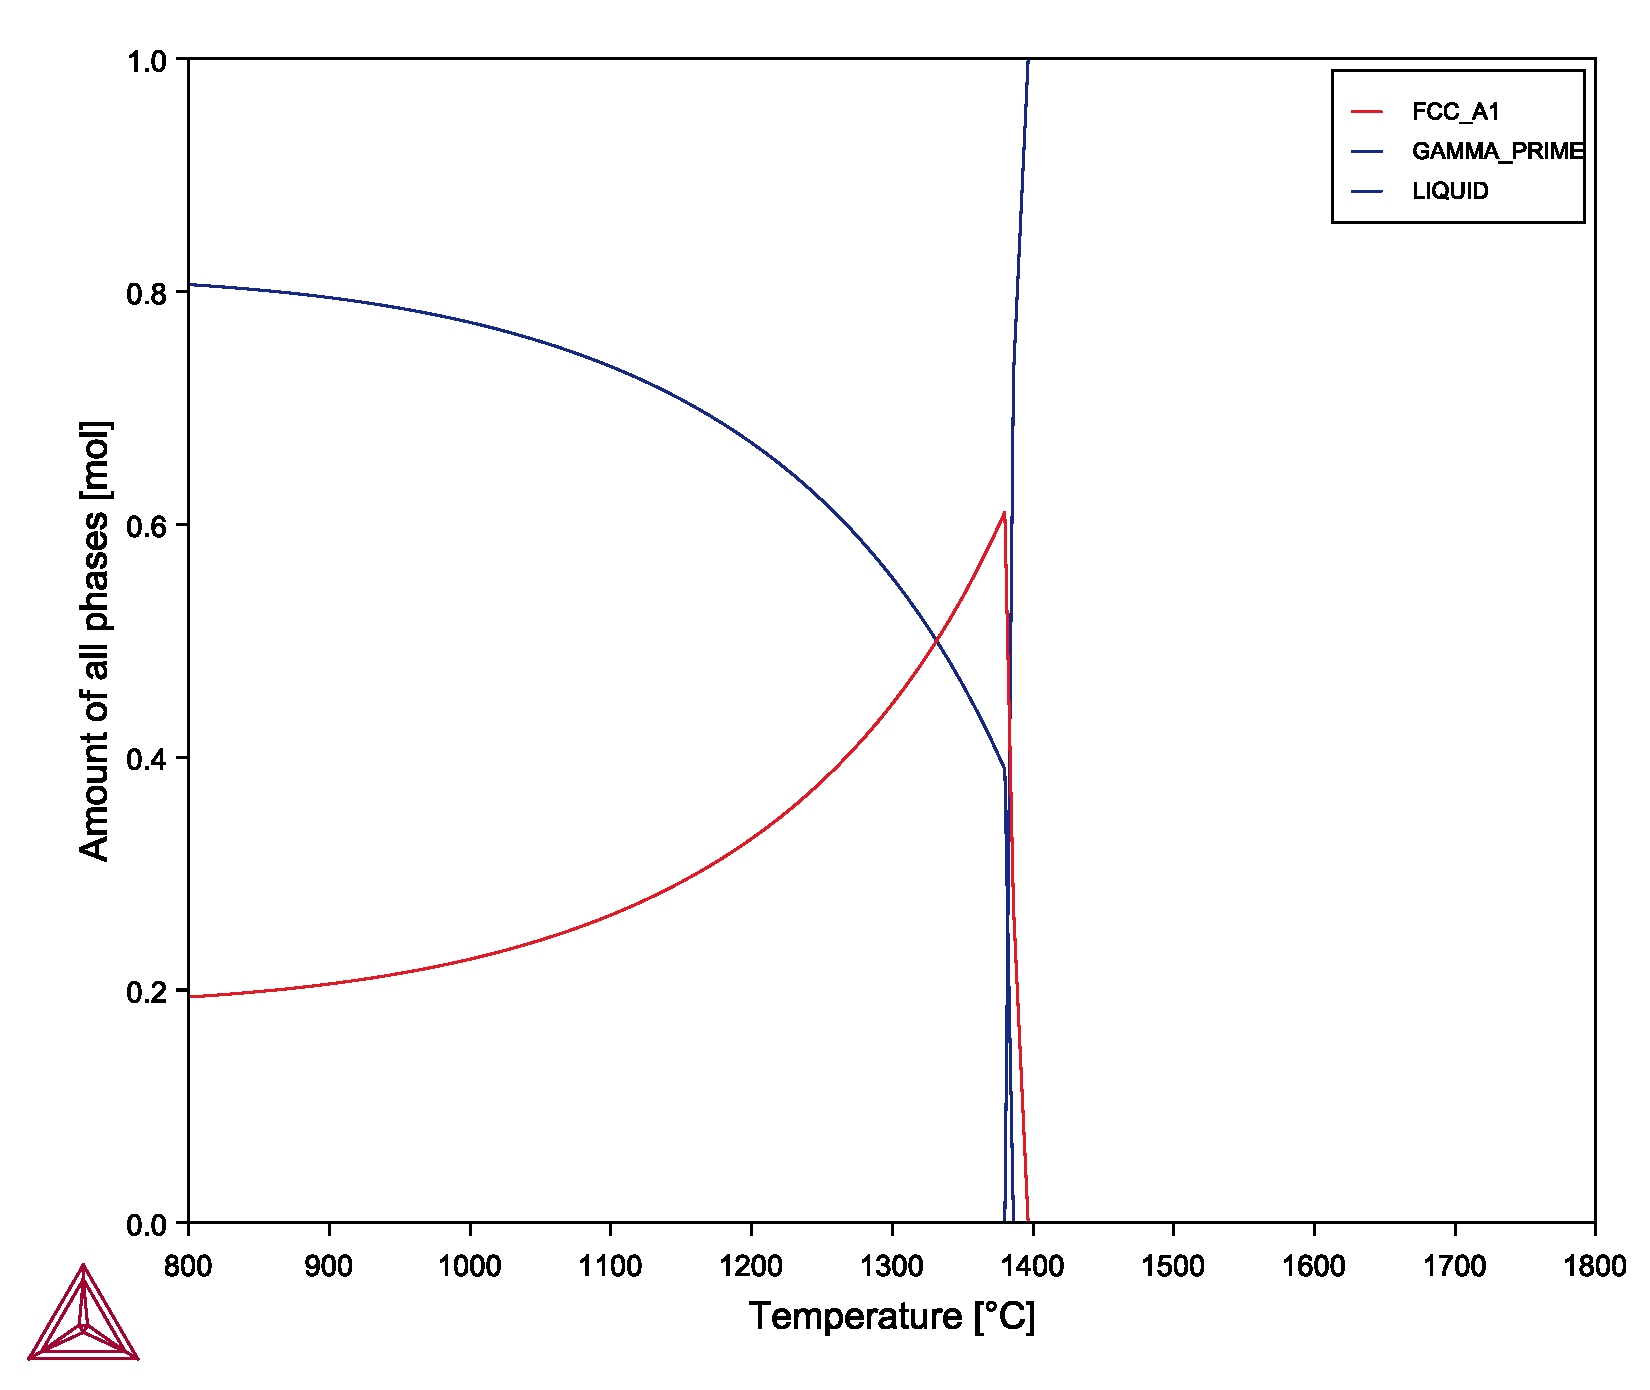
\includegraphics[width=0.95\textwidth]{graficas/Q4_02.pdf}
    \caption{Amount of all phases as a function of temperature generated with \textit{ThermoCalc} \citep{thermocalc}}
    \label{fig:diagram05}
\end{figure}

The primary ageing temperature is found at a $\gamma'$ fraction of approximately 0.60, this is following the gamma prime curve 

%The γ′ fraction at lower temperatures is used to define the ageing condition. From the diagram, the γ′ fraction reaches ≈0.60 at a temperature of about 1080 °C. This temperature is therefore selected as the primary ageing temperature, where a stable amount of precipitates can form and strengthen the alloy.

